\begin{figure}
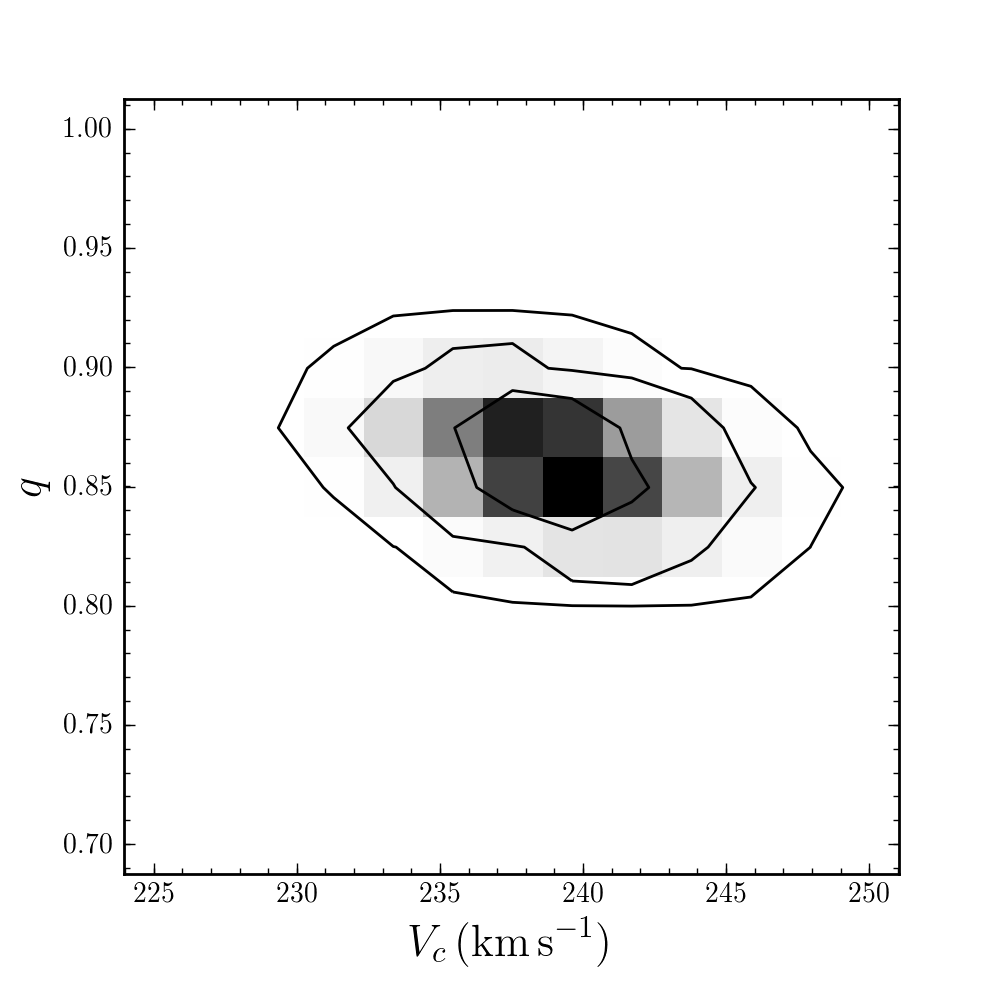
\includegraphics[width=83mm]{./figures/jo_results.png}
  \caption{Jo's results (Sec.~\ref{ssec:jo_results})}
  \label{plot_jo_results}
\end{figure}

\begin{figure}
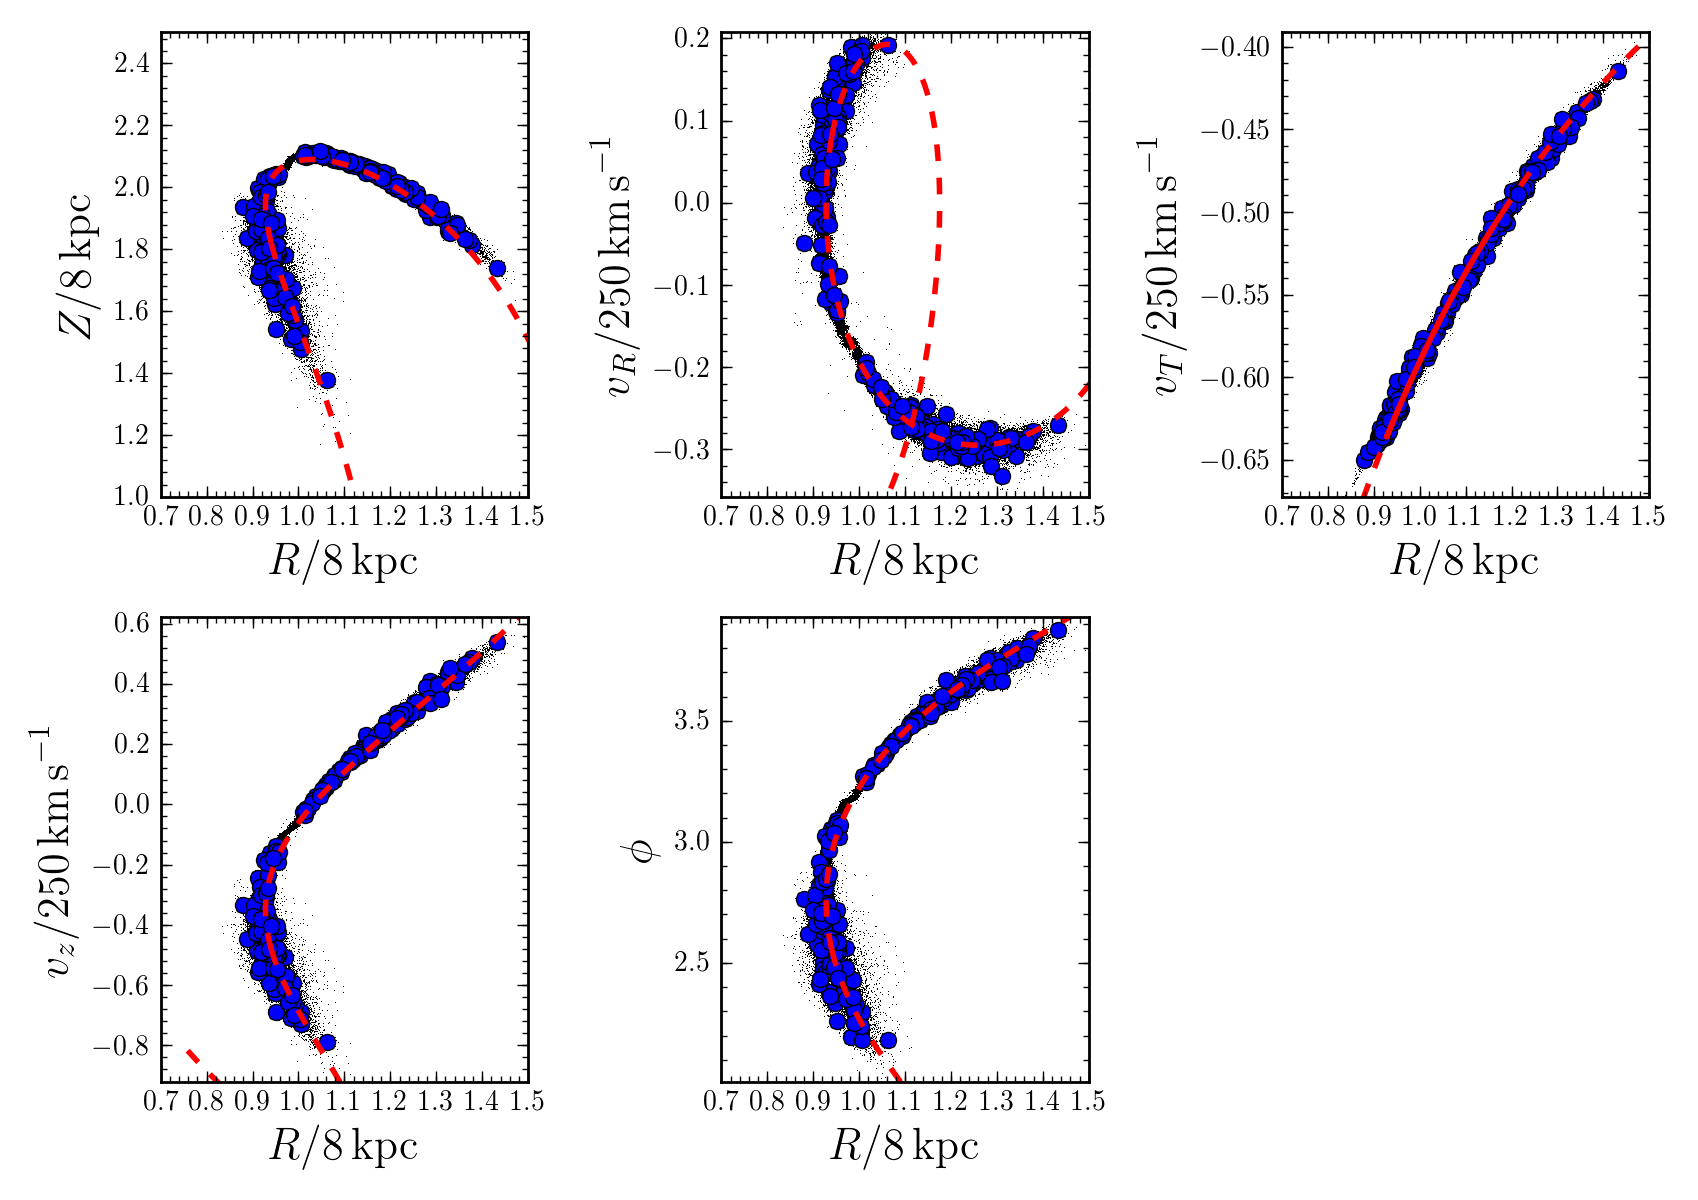
\includegraphics[width=83mm]{./figures/jo_orbitfit.png}
  \caption{Jo's results (Sec.~\ref{ssec:jo_results})}
  \label{plot_jo_orbitfit}
\end{figure}

I computed the acceleration at Pal 5 and get
$a(Pal5) = 3.42 \pm 0.04 pc/Myr^2$.

The PDF in Fig.~\ref{plot_jo_results} shows 1, 2, and 3 sigma contours. 
I just fit a flattened logarithmic potential, so the PDF is for those two parameters ($v_c$ and flattening $q$). 
The orbit fit in Fig.~\ref{plot_jo_orbitfit} shows different projections: I fit to the 200 blue points, the best-fitting orbit is shown in red.
